\documentclass[10pt,a4paper]{article}
\usepackage[utf8]{inputenc}
\usepackage[danish]{babel}
\usepackage{amsmath}
\usepackage{amsfonts}
\usepackage{amssymb}
\usepackage{graphicx}
\usepackage[left=2cm,right=2cm,top=2cm,bottom=2cm]{geometry}


\usepackage{titlepic}
\usepackage{enumerate}
\usepackage{enumitem}
\usepackage{float}
\usepackage{pdfpages}
\usepackage[colorlinks = true,
            linkcolor = blue,
            urlcolor  = blue,
            citecolor = blue,
            anchorcolor = blue]{hyperref}
\usepackage[explicit]{titlesec}
\usepackage{pstricks}
\usepackage[amsmath,thmmarks]{ntheorem} %pakke til at lave sætningsenvorinmets (kan ikke loades sammen med amsthm)
\usepackage{color}
\usepackage{tikz}

%opretter environmets til sætningsstrukturen 
\theorembodyfont{\normalfont}

	
	%sætnings environment	
	\newtheorem{thm}{Sætning}

	\theoremstyle{break}	
	%opgave environment	
	\newtheorem{opg}{Opgave}	

	%Korrolar environment
	\newtheorem{korollar}[thm]{Korollar}	
	
	%Lemma environment	
	\newtheorem{lemma}[thm]{Lemma}
	
	\theoremsymbol{\ensuremath{\circ}}	
	
	%definition environment	
	\newtheorem{definition}[thm]{Definition}
	
	%eksempel environment	
	\newtheorem{eksempel}[thm]{Eksempel}
	
	
	
	%Bevis environment
	\theoremstyle{nonumberplain}
	\theoremheaderfont{%
	\normalfont\itshape}
	\theorembodyfont{\normalfont}
	\theoremsymbol{\ensuremath{\square}}
	\theoremseparator{.}
	
	\newtheorem{proof}{Bevis}
	\newtheorem{los}{Løsning}
	






\setlength\parindent{0pt}

%\titleformat{\section}{\Large\bfseries}{}{0pt}{#1}
%\titleformat{\subsection}{\large\bfseries}{}{0pt}{#1}


%nye komandoer
\newcommand{\mR}{\mathbb{R}}
\newcommand{\mZ}{\mathbb{Z}}
\newcommand{\mN}{\mathbb{N}}
\newcommand{\mQ}{\mathbb{Q}}
\newcommand{\mC}{\mathbb{C}}
\newcommand{\hs}{\hspace{2mm}}
\newcommand{\Hs}{\hspace{4mm}}
\newcommand{\pipe}{\hs | \hs}
\newcommand{\lp}{\left(}
\newcommand{\rp}{\right)}
\newcommand{\vect}[1]{\underline{#1}}
\newcommand{\matr}[1]{\underline{\underline{#1}}}
\newcommand{\cnum}[1]{\raisebox{.5pt}{\textcircled{\raisebox{-.9pt} {#1}}}}




\author{Mikkel B. Goldschmidt\\3r, Nørre Gymnasium}
\title{Laplace lov}
\date{\today}



\begin{document}
\maketitle

\section{Indledning}
Laplaces lov beskriver den kraft, F, der påvirker en elektrisk leder leder med længde, l, hvorigennem der løber en strøm med styrke I, der er anbragt i et magnetfelt med styrke, B, med en vinkel $\Theta$ mellem magnetfeltet og lederen.

Den siger at: 
$$F=B \cdot I \cdot L\cdot \sin (\theta)$$

\section{Teori}
Laplace lov som den vil blive behandlet i denne rapport, er udelukkende en empirisk begrundet lov. 
Dog har den nogle interessante følger i forhold til kraften på elektroner og andre ladede partikler i et magnetfelt, som jeg vil behandle i et perspektiverende afsnit. 

Laplace lov er lidt mere beskrivende en den form jeg beskrev i indledningen. 
Hvis man betragter kraften, strømmen retning og magnetfeltet som vektorer $\overrightarrow{F}$, $\overrightarrow{l}$ og $\overrightarrow{B}$.
Bemærk at magnetfeltet egentlig er et vektorfelt, men at alle relevante vektorer i feltet er lig hinanden da vi arbejder i et homogent magnetfelt. 
Vi kan derfor tillade os at behandle det som en vektor $\overrightarrow{B}$, som er lig en vilkårlig vektor i vektorfeltet. 

Den lov vi vil eftervise er beskrevet med vektorer på følgende måde:
\newcommand{\vek}[1]{\overrightarrow{#1}}

$$\vek{F} = I\cdot (\vek{l}\times \vek{B})$$

Ved at huske at der for krydsproduktet af to vilkårlige vektorer,$\vek{v}$ og $\vek{u}$ med vinkel $\theta$ mellem sig, at 

$|\vek{v} \times \vek{u}|=|\vek{v}|\cdot |\vek{u}| \cdot \sin (\theta)$ ved vi altså at den ovenfor angivne sammenhæng angiver den samme længe af vektor $\vek{F}$ som den første formel, den angiver også bare en længde.

I dette forsøg kommer vi kun til at kigge på et scenarie hvor $\theta=90$. 
Derfor vil kraften altid have samme retning og $\sin (\theta) = 1$ og vi får altså bare en sammenhæng på formen:
$$F = B\cdot I\cdot L$$
som vi vil undersøge.

\pagebreak  
\section{Forsøgsbeskrivelse}
Vi udførte tre forsøg til at bekræfte loven. 
I alle tre forsøg har vi haft en ''Hestesko''-magnet anbragt på en vægt. 
Ned imellem de to poler nede i hesteskoen, satte vi en elektrisk fastsat på en plade der var sat i et stativ.
Gennem denne leder løb der jævnstrøm, der kunne justeres fra en strømforsyning. 
I serieforbindelse mellem strømforsyningen og og lederen var et amperemeter placeret.
På figur \ref{opstilling} kan ses et billede af den beskrevne opstilling.	


\begin{figure}[h]
\center
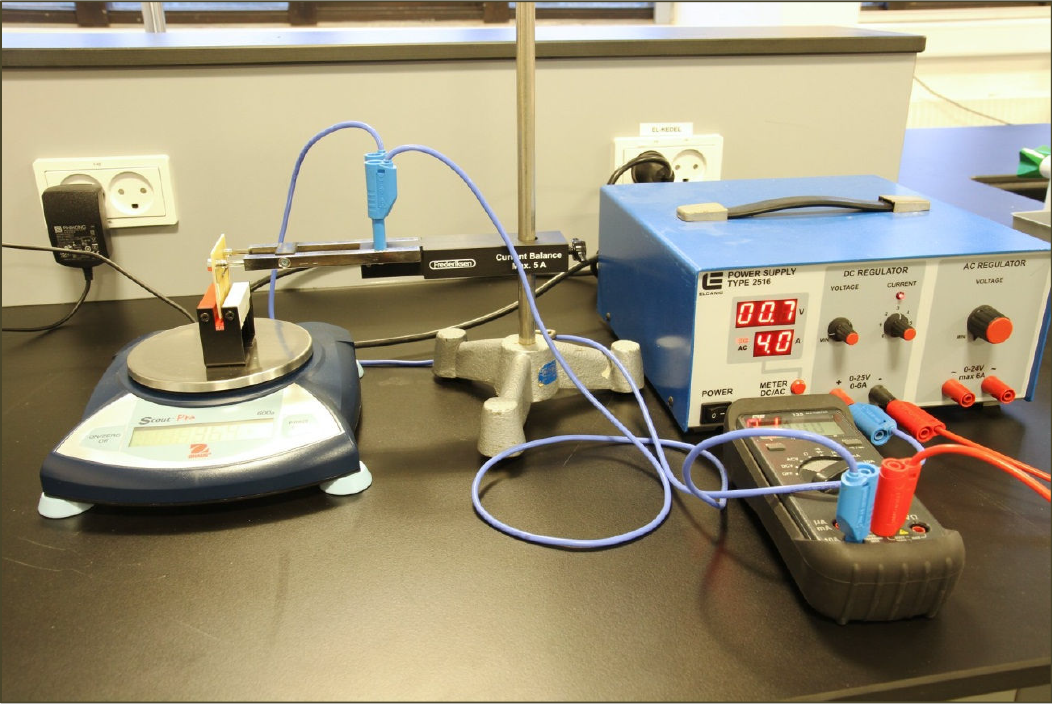
\includegraphics[scale=0.4]{opstilling}
\caption{Et billede af forsøgsopstillingen for alle tre delforsøg. Billedet er taget af Erik Westergaard fra www.matematikogfysik.dk}
\label{opstilling}
\end{figure}

Vi lavede da tre måleserier hvor vi kiggede på ændringen i $F$, når vi varierede henholdsvis $B,I$ og $L$, mens vi holdt de andre konstante. 
\pagebreak
\section{Data}
I alle tre delforsøg har vi målt en vægt som aflæst på vægten. 
Ud fra denne vægt har vi beregnet en kraft, ud fra at $F = m \cdot g$, hvor $9.82 \frac{N}{kg}$.
\subsection{I,F - måleserie}
Vi målte her vægten $m$ i forhold til strømstyrken gennem lederen $I$:

\begin{table}[h]
\centering
\begin{tabular}{|l|ll|}
\hline
\textbf{$I (A)$} & \textbf{$m(g)$} & \textbf{$F(mN)$} \\ \hline
0                & 165,11          & 1,0802          \\
0,38             & 164,95          & 2,6514          \\
0,41             & 164,94          & 2,7496          \\
0,55             & 164,87          & 3,437           \\
0,66             & 164,83          & 3,8298          \\
0,76             & 164,79          & 4,2226          \\
0,89             & 164,73          & 4,8118          \\
1,09             & 164,65          & 5,5974          \\
1,22             & 164,59          & 6,1866          \\
1,3              & 164,56          & 6,4812          \\
1,48             & 164,48          & 7,2668          \\
1,67             & 164,4           & 8,0524          \\
1,96             & 164,27          & 9,329           \\
2,28             & 164,14          & 10,6056         \\
2,64             & 163,98          & 12,1768         \\
2,99             & 163,84          & 13,5516         \\
3,25             & 163,72          & 14,73           \\
3,36             & 163,67          & 15,221          \\
3,47             & 163,63          & 15,6138         \\
3,78             & 163,49          & 16,9886         \\
3,83             & 163,48          & 17,0868         \\
3,98             & 163,41          & 17,7742         \\
\hline

\end{tabular}
\caption{Delforsøg 1. Snorens længde var $3.2 cm$.}
\end{table}

\pagebreak
\subsection{L, F - Måleserie}
Vi målte her vægten i forhold til længden af lederen. 
Bemærk at vægten har været nulstillet inden målingerne, og vi har derfor kun regnet massedifferenser. 

\begin{table}[h]
\centering

\begin{tabular}{|l|ll|}
\hline
\textbf{Længde ($cm$)} & \textbf{Masse($g$)} & \textbf{Kraft ($mN$)} \\ \hline
1,2                    & -0,43               & 4,2226                \\
2,2                    & -0,71               & 6,9722                \\
3,2                    & -0,96               & 9,4272                \\
4,2                    & -1,22               & 11,9804               \\
6,4                    & -1,82               & 17,8724               \\
8,4                    & -2,3                & 22,586               \\
\hline
\end{tabular}
\caption{Delforsøg 2. Strømstyrken var $2.04A$.}
\end{table}

\subsection{B, F - Måleserie}
I dette forsøg har vi varieret antallet af magneter. 
Da det magnetfelt de skaber er ukendt, har vi blot noteret antallet af magneter.

\begin{table}[h]
\centering

\begin{tabular}{|l|ll|}
\hline
\textbf{Magneter ($B$)} & \textbf{Masse($m$)} & \textbf{Kraft($mN$)} \\ \hline
1                       & 12,33               & 6,1866               \\
2                       & 24,67               & 12,275               \\
3                       & 37,07               & 17,7742              \\
4                       & 49,57               & 22,2914              \\
5                       & 62,06               & 26,9068              \\
6                       & 74,65               & 30,5402   			\\
\hline          
\end{tabular}

\caption{Delforsøg 3. Strømstyrken var $2.01 A$, og lederens længde var $8.4cm$.}
\end{table}

\section{Databehandling}
Da vi forventer en lineær sammenhæng i alle tre tilfælde, tegner jeg grafer for disse og laver en lineær regression:
\subsubsection{Delforsøg 1}
\begin{center}
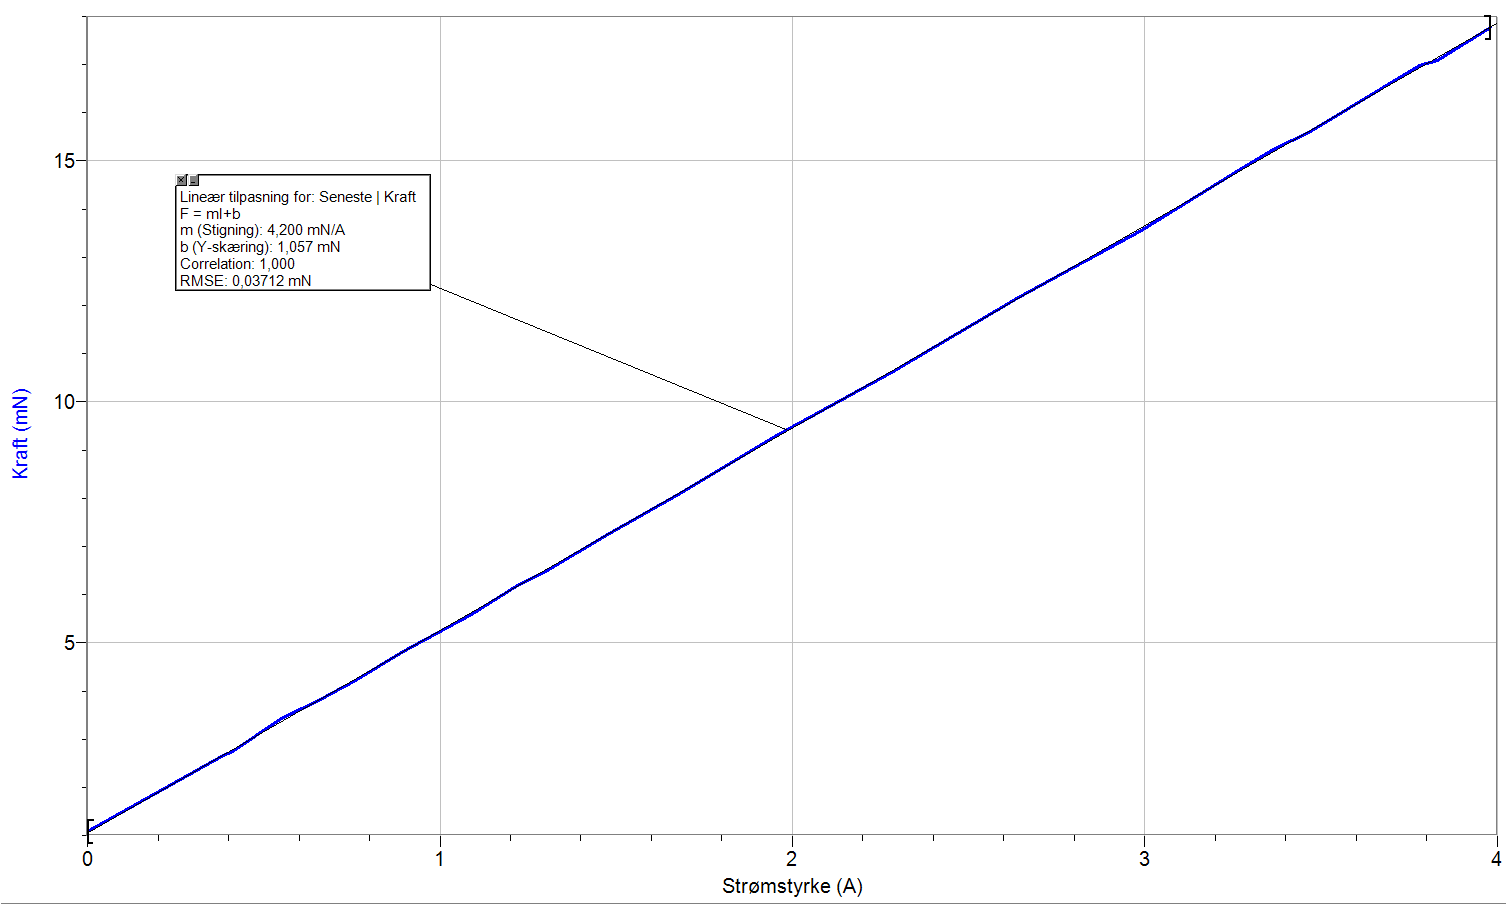
\includegraphics[scale=0.5]{graf1}
\end{center}

\subsubsection{Delforsøg 2}
\begin{center}
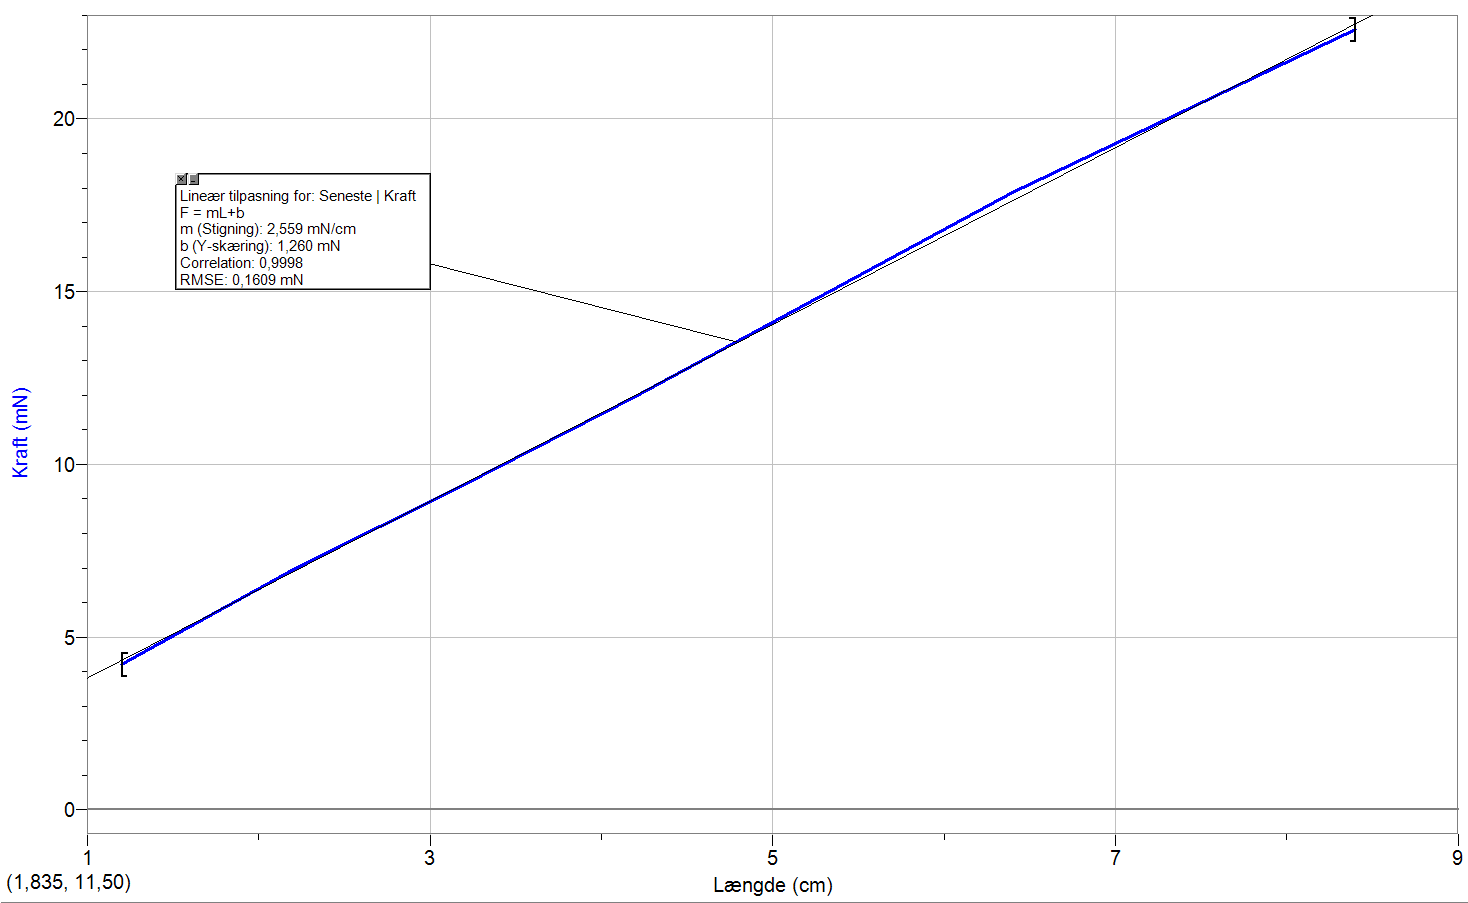
\includegraphics[scale=0.5]{graf2}
\end{center}

\subsubsection{Delforsøg 3}
\begin{center}
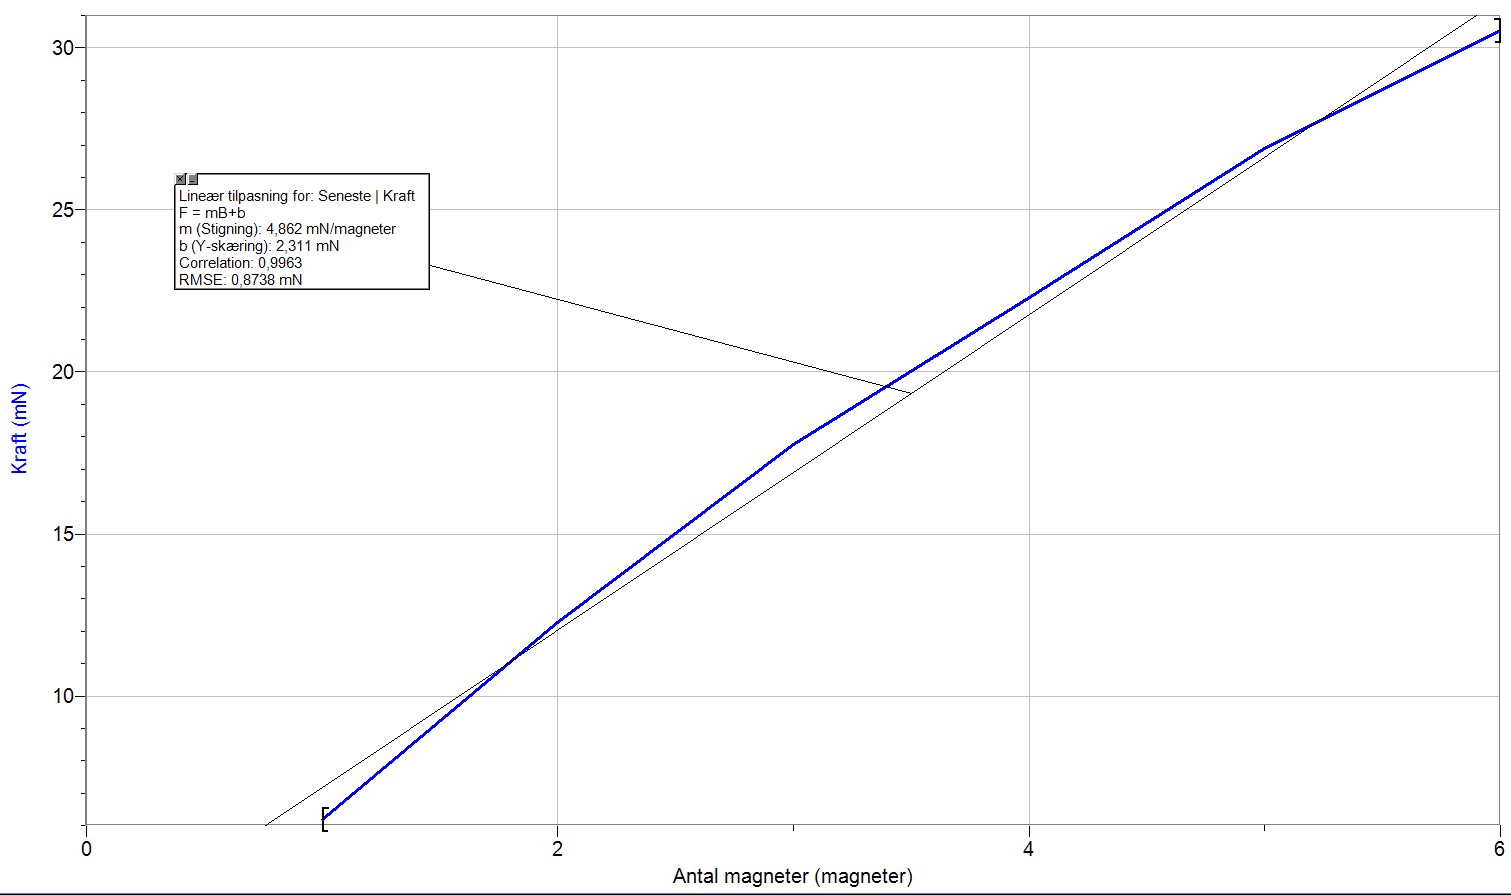
\includegraphics[scale=0.5]{graf3}
\end{center}

\subsection{Fundne sammenhænge}
I delforsøg nr. 1 fås sammenhængen: $F=4.200\frac{mN}{A}*I+1.057mN$.

I delforsøg nr. 2 fås sammenhængen : $F = 2.559\frac{mN}{cm}*L + 1.260mN$.

I delforsøg nr. 3 fås sammenhængen $F = 4.862mN\cdot n + 2.311 mN$, hvor $n$ repræsenterer antallet af små magneter, hvoraf der i alt skulle 6 til at udgøre den magnet der er brugt i de andre delforsøg. 

Jeg vil nu undersøge, hvor godt resultaterne passer med Laplace lov. 
Dette vil jeg gøre ved at beregne magnetfeltets størrelse $B$ i hvert af de tre forsøg.

\subsubsection{Delforsøg 1: Bestemmelse af $B$}
Den fundne sammenhæng I delforsøg nr. 1 var: $F=4.200\frac{mN}{A}\cdot I+1.057mN$. 
Først ser vi bort fra konstantledet, da dette kun er på for at tage højde for en vægt som magneten har påvirket vægten med.
Vi har da sammenhængen $F=4.200\frac{mN}{A}\cdot I$. 
Ved Laplace lov får vi at $F=B\cdot L \cdot I$ og dermed 
$B\cdot L = 4.200\frac{mN}{A}$. 

Da kan vi beregne $B$ som $\dfrac{4.200\frac{mN}{A}}{L}$.
Vi ved som beskrevet i dataafsnittet af $L=3.2cm$. 
Vi kan da beregne en værdi for $B$:
$$B = \dfrac{4.200\frac{mN}{A}}{L} = \dfrac{4.200\frac{mN}{A}}{3.2cm} = 0.13T$$

\subsubsection{Delforsøg 2: Bestemmelse af $B$}
Den fundne sammenhæng i dette delforsøg er $F = 2.559\frac{mN}{cm}*L + 1.260mN$.
Ligesom i forrige afsnit ser vi bort fra konstantledet.
Vi kan da med et argument på samme måde som i forrige afsnit se at $B=\dfrac{2.559\frac{mN}{cm}}{I}$. 
I dataafsnittet kan ses at $I=2.04A$.

$$B = \dfrac{2.559\frac{mN}{cm}}{I}  = \dfrac{2.559\frac{mN}{cm}}{2.04A} = 0.12T$$

\subsubsection{Delforsøg 3: Bestemmelse af $B$}
Dette forsøg er lidt anderledes end de andre.
Først ser vi dog at vi ligesom i de andre forsøg bør fjerne konstantleddet: $F = 4.862mN\cdot n$ med $n$ værende antallet af små magneter. 
 
Vi vil her forvente at $B$ kan bestemme $B$ som et produkt af alle de små magneter der skulle til for at ave hele magneten. 
Hvis vi kalder magnetfeltsstyrken fra en af de små magneter der skulle til at lave den store for $B_1$, vil vi da forvente af $B=6B_1$, da den store magnet var lavet af $6$ små.
Da vi med Laplace lov har at $F=BIL$ og magnetfeltstyrken afhænger af $n$ som $B=n\cdot B_1$, forventer vi altså $F=n\cdot B_1 \cdot I \cdot L$.
Da vi fra forsøget har $F=4.862mN\cdot n$, må vi ved at kombinere de to få: 
$B_1 \cdot I \cdot L = 4.862mN$.
Da vi har fra datasektionen at $I=2.01A$ og $L=8.4cm$, får vi altså 
$$B_1 = \dfrac{4.862mN}{2.01 A\cdot 8.4 cm}=2.9\cdot 10^{-2}T$$
Da kan $B$ beregnes:
$$B = 6 B_1 = 6\cdot 2.9\cdot 10^{-2}T=0.18T$$

\subsection{Vurdering af resultater}
De tre resultater er nogenlunde ens. 
Specielt er værdien af $B$ i forsøg 1 og 2 meget tæt på hinanden, hvilket styrker hypotesen om at Laplace lov er sand. 
Dog er det værd at bemærke, at værdien fra delforsøg 3 varierer fra de to andre.
Det giver dog også god mening da data fra forsøg 3 er markant dårligere end i de to andre (se grafen til forsøg 3 som ikke ser fuldstændig lineær ud). 
Den dårligere data er også forståelig da vi i dette forsøg forsøger at kontrollere styrken af et magnetfelt. 
Selvom magnetfeltet imellem benene på en hesteskomagnet er tilnærmelsesvist lineært, så kan det godt opstå udforudsete ting når vi ændrer på det. 
Man kunne måske tænke at magneten påvirker lederen med den del af dets magnetfelt som ikke er mellem benene. 
Generelt er det bare svært at forudsige præcist hvordan magnetfelter opfører sig, og derfor giver urenhederne i vores data god mening. 

\section{Konklusion}
Forsøgene ser ud til at bekræfte at Laplace lov gælder. 
Selvom der er små urenheder i vores data, der ikke helt stemmer overens med teorien perfekt, så kan disse bortforklares nogenlunde rimeligt. 
Vi kan derfor konkludere at observationerne ikke strider imod Laplace lov.




\end{document}